\documentclass{beamer}

\usepackage{Vor2018glærur}

\title{Tölvunarfræði 2}
\subtitle{Vika 11}

\begin{document}

\begin{frame}
	\titlepage
\end{frame}

\section{Hagnýting neta}

\imageslide{AlgsSlides/graph-applications}

\imageslide{AlgsSlides/graph-states-usa}

\imageslide{AlgsSlides/graph-facebook-friends}

\begin{frame}{Facebook graph API}
	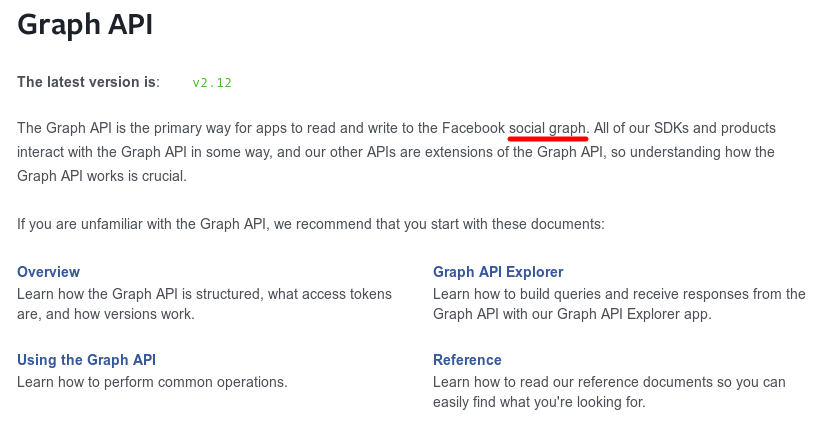
\includegraphics[width=\textwidth]{graph-api-facebook}

	\begin{center}
		\url{https://developers.facebook.com/docs/graph-api/}
	\end{center}
\end{frame}

\begin{frame}{Tengsl forrita}
	Pakkakerfi: \url{https://anvaka.github.io/pm/}
\end{frame}

\imageslide{AlgsSlides/graph-protein-interaction}

\section{Stærðfræðilegur bakgrunnur}

\begin{frame}{Óstefnt net}
	\begin{columns}
		\column{0.65\textwidth}
		\begin{tcolorbox}[title=Óstefnt net]
			Óstefnt net \eng{undirected graph} $G = (V, E)$ samanstendur af tveimur mengjum, $V$, ekki-tómu mengi hnúta (e.\ \emph{vertices} eða \emph{nodes}) og $E$, mengi leggja \eng{edges}. Hver leggur er tengdur við einn eða tvo hnúta, sem eru endahnútar \eng{endpoints} leggsins.
		\end{tcolorbox}
		\column{0.35\textwidth}
		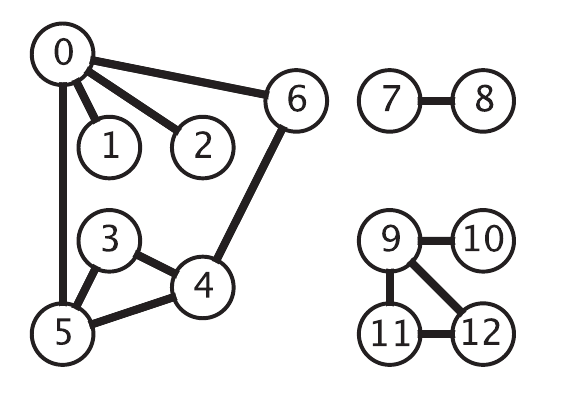
\includegraphics[width=\linewidth]{tinyg}

		\begin{center}
			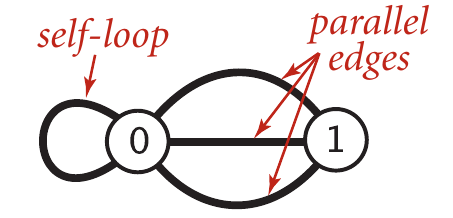
\includegraphics[width=0.7\linewidth]{graph-multipseudograph}
		\end{center}
	\end{columns}
\end{frame}

\imageslide{AlgsSlides/graph-drawing}

\begin{frame}{Hugtök}
	\begin{itemize}
		\item Tveir hnútar $u$ og $v$ í óstefndu neti $G$ eru aðlægir \eng{adjacent} ef bæði $u$ og $v$ koma fyrir í skilgreiningu einhvers leggs í $G$
		\item Nágrannar \eng{neighbours} hnúts $v$ eru þeir hnútar sem eru aðlægir $v$
		\item Lykkja \eng{loop} er leggur sem tengdur er við einn hnút
		\item Stig \eng{degree} hnúts $v$ í óstefndu neti er fjöldi hnúta sem eru aðlægir $v$
		      \begin{itemize}
			      \item Lykkja á hnút ``telur tvöfalt'', hækkar stig hnútsins um 2
			      \item Stig hnúts $v$ er táknað með $\deg(v)$
		      \end{itemize}
	\end{itemize}
\end{frame}

\begin{frame}{Gerðir óstefndra neta}
	\begin{itemize}
		\item Við getum flokkað óstefnd net eftir því hvers konar leggi við leyfum
		      \begin{itemize}
			      \item Net sem leyfir marga leggi á milli tveggja hnúta er kallað fjölnet \eng{multigraph}
			      \item Net sem leyfir lykkjur er (stundum) kallað gervinet \eng{pseudograph}
			      \item Net sem leyfir hvorki lykkjur né endurtekna leggi er kallað einfalt net \eng{simple graph}
		      \end{itemize}
		\item Tökum fram hvað við eigum við þegar það skiptir máli
	\end{itemize}
\end{frame}

\begin{frame}{Handabandssetningin}
	\begin{tcolorbox}[title=Handabandssetningin]
		Látum $G = (V, E)$ vera óstefnt net með $m$ leggjum. Þá er
		\[
			2m = \sum_{v \in V} \deg(v)
		\]
	\end{tcolorbox}
	Handabandssetningin \eng{the handshake theorem} á við um fjölnet og net með lykkjum.
\end{frame}

\begin{frame}{Grennslafylki}
	Látum $G = (V, E)$ vera einfalt net með $|V| = n$ og búum til röðun á hnútunum $v_1, v_2, \ldots v_n$. Grennslafylkið $A_G$ m.t.t. þessarar röðunar er þá $n \times n$ fylki $[a_{ij}]$ þar sem $a_{ij}$ er 1 sé $\{v_i,v_j\}$ leggur í netinu og 0 annars.

	Dæmi, með hnútaröðunina í stafrófsröð:
	\begin{columns}
		\column{0.2\textwidth}
		\begin{center}
			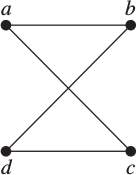
\includegraphics[width=\linewidth]{graph-mini}
		\end{center}
		\column{0.3\textwidth}
		\[
			A =
			\begin{bmatrix}
				0 & 1 & 1 & 0 \\
				1 & 0 & 0 & 1 \\
				1 & 0 & 0 & 1 \\
				0 & 1 & 1 & 0 \\
			\end{bmatrix}
		\]
	\end{columns}
	\vspace{0.2cm}
	Væri netið ekki einfalt gætum við sett hærri tölur í sætin.
\end{frame}

\begin{frame}{Fjöldi vega}
	\begin{tcolorbox}
		Látum $G$ vera net með grennslafylkið $A$ m.t.t. hnútaröðunar $v_1, \ldots, v_n$. Þá er fjöldi mismunandi vega af jákvæðri lengd $r$ á milli hnúta $v_i$ og $v_j$ talan sem er í sæti $i,j$ í fylkinu $A^r$.
	\end{tcolorbox}
	\begin{columns}
		\column{0.2\textwidth}
		\begin{center}
			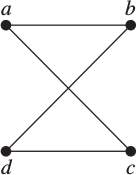
\includegraphics[width=\linewidth]{graph-mini}
		\end{center}
		\column{0.6\textwidth}
		\[
			A =
			\begin{bmatrix}
				0 & 1 & 1 & 0 \\
				1 & 0 & 0 & 1 \\
				1 & 0 & 0 & 1 \\
				0 & 1 & 1 & 0 \\
			\end{bmatrix}
			,
			A^4 =
			\begin{bmatrix}
				8 & 0 & 0 & 8 \\
				0 & 8 & 8 & 0 \\
				0 & 8 & 8 & 0 \\
				8 & 0 & 0 & 8 \\
			\end{bmatrix}
		\]
		\begin{center}
			Svo fjöldi mismunandi vega á milli t.d. $a$ og $d$ af lengd 4 er 8.
		\end{center}
	\end{columns}
\end{frame}

\section{Útfærsla á óstefndum netum}

\imageslide{AlgsSlides/graph-api}

\begin{frame}{Hvernig skal geyma net í tölvu?}
	\begin{itemize}
		\item Ekki endilega augljóst hvernig best sé að útfæra klasa fyrir óstefnt net
		      \begin{itemize}
			      \item Grennslafylki
			            \begin{itemize}
				            \item Þarf að geyma $|V|^2$ rökgildi, skalast illa
			            \end{itemize}
			      \item ``Node'' klasi með vísunum í aðlæga hnúta
			            \begin{itemize}
				            \item Flókið, ekkert ``random access'' að upplýsingum um nágranna
			            \end{itemize}
			      \item Geymum einvítt fylki af pörum sem tákna leggi
			            \begin{itemize}
				            \item Erfitt að finna nágranna hnúts
			            \end{itemize}
		      \end{itemize}
		\item Það sem oftast er gert: Geyma fylki af grennslalistum \eng{adjacency lists}
	\end{itemize}
\end{frame}

\imageslide{AlgsSlides/graph-adjacency-list}

\imageslide{AlgsSlides/graph-sparse-dense}

\imageslide{AlgsSlides/graph-symbol}

\imageslide{AlgsSlides/graph-java-implementation}

\section{Leit í netum}

\imageslide{AlgsSlides/graph-paths}

\imageslide{AlgsSlides/graph-maze}

\imageslide{AlgsSlides/graph-maze-exploration}

\imageslide{AlgsSlides/graph-dfs}

\imageslide{AlgsSlides/graph-dfs-data}

\imageslide{AlgsSlides/graph-dfs-java}

\imageslide{AlgsSlides/graph-dfs-properties}

\imageslide{AlgsSlides/graph-dfs-xkcd}

\imageslide{AlgsSlides/graph-bfs}

\imageslide{AlgsSlides/graph-bfs-dfs}

\imageslide{AlgsSlides/graph-bfs-java}

\imageslide{AlgsSlides/graph-communication}

\imageslide{AlgsSlides/graph-erdos}

\section{Stefnd net}

\begin{frame}{Stefnt net}
	\begin{tcolorbox}[title=Stefnt net]
		Stefnt net (e. \emph{directed graph}) samanstendur af mengi $V$ af hnútum og mengi $E$ af röðuðum pörum af hnútum í $V$ sem nefnast stefndir leggir (e. \emph{directed edges}). Í leggnum $(a, b)$ er fyrri hnúturinn upphafshnútur (e. \emph{initial vertex}) og seinni hnúturinn lokahnútur (e. \emph{terminal vertex}).
	\end{tcolorbox}

	Getum lýst einföldum stefndum netum, stefndum fjölnetum og stefndum lykkjum á svipaðan hátt og við gerðum fyrir óstefndu netin.

	Stefndir leggir eru líka kallaðir örvaleggir.
\end{frame}

\imageslide{AlgsSlides/digraph-example}

\imageslide{AlgsSlides/digraph-map}

\imageslide{AlgsSlides/digraph-api}

\imageslide{AlgsSlides/digraph-usage}

\imageslide{AlgsSlides/digraph-adjacency-list}

\imageslide{AlgsSlides/digraph-java}

\section{Lok}

\begin{frame}{Þessi glærupakki}
	Kóða fyrir algs4 reiknirit má finna á \url{http://algs4.cs.princeton.edu/code/}.

	Glærur með gráan bakgrunn má finna á \url{https://algs4.cs.princeton.edu/lectures/}.

	Gagnaskrár má finna á \href{https://github.com/Ernir/kennsluefni/tree/master/T2/Code/w11}{Github} og algs4-data.zip.
\end{frame}

\begin{frame}{Næst}
	Spanntré (kafli 4.3), vegin net (kafli 4.4).
\end{frame}

\end{document}
